% Generated by paper/tables/strengthen_tables.py. Do not edit by hand.
\section{Confirmation campaign: full tables}\label{app:confirm}
This appendix expands \cref{sec:confirm}. \Cref{tab:strengthen-factorial-full} expands \cref{tab:strengthen-factorial} to all eight contrasts and ten metrics; \cref{tab:strengthen-factorial-means} gives the factorial cell means; \cref{tab:strengthen-sweep,fig:fs-sweep} give the temperature sweep; \cref{tab:strengthen-fresh-arms} compares every fresh-prompt arm with \segaofficial; \cref{tab:strengthen-seeds} gives the seed replication; \cref{tab:strengthen-ckpt} the checkpoint-by-guidance lattice; \cref{tab:strengthen-default-shift} the default flow shift. Every table lists all registered metrics, including unfavourable ones, with nominal 95\% paired prompt-bootstrap intervals (2{,}000 draws, seed 0).

% Generated by paper/tables/strengthen_tables.py. Do not edit by hand.
\begin{table}[!htbp]
\centering
\caption{\textbf{All factorial contrasts.} Every registered contrast and metric of the held-out factorial ($n=187$, seed 0), with the same cells, marks and Holm family as \cref{tab:strengthen-factorial}, transposed; bold marks the largest gain for each metric. Key result: 31 of 80 tests survive Holm: 27 temperature tests (every metric except tiling) and 4 allocation tests (better on full-frame MUSIQ, crop CLIP-IQA and slope error; worse on tiling); neither the RoPE base nor the interaction survives Holm on any of the ten metrics.}
\label{tab:strengthen-factorial-full}
\scriptsize
\setlength{\tabcolsep}{1.8pt}
% Generated by paper/tables/strengthen_tables.py. Do not edit by hand.
% Caption: \textbf{All factorial contrasts.} Every registered contrast and metric of the held-out factorial ($n=187$, seed 0), with the same cells, marks and Holm family as \cref{tab:strengthen-factorial}, transposed; bold marks the largest gain for each metric. Key result: 31 of 80 tests survive Holm: 27 temperature tests (every metric except tiling) and 4 allocation tests (better on full-frame MUSIQ, crop CLIP-IQA and slope error; worse on tiling); neither the RoPE base nor the interaction survives Holm on any of the ten metrics.
\begin{tabular}{@{}lrrrr@{}}
\toprule
\emph{Main effects} & \hdr{Base\\(main)} & \hdr{Temperature\\(main)} & \hdr{Base $\times$\\temp.} & \hdr{Allocation\\\phantom{x}} \\
\midrule
ImageReward$\uparrow$ & \dcellT{+0.027}{-0.003}{+0.056} & \dcellB{+0.594^{*}}{+0.506}{+0.686} & \dcellT{-0.018}{-0.087}{+0.047} & \dcellT{-0.026}{-0.068}{+0.014} \\
PickScore$\uparrow$ & \dcellT{+0.02}{-0.03}{+0.06} & \dcellB{+1.04^{*}}{+0.92}{+1.16} & \dcellT{+0.00}{-0.07}{+0.08} & \dcellT{-0.03}{-0.09}{+0.03} \\
CLIP$\uparrow$ & \dcellT{-0.02}{-0.15}{+0.11} & \dcellB{+2.03^{*}}{+1.61}{+2.47} & \dcellB{+0.38}{+0.12}{+0.66} & \dcellT{-0.02}{-0.23}{+0.19} \\
MUSIQ$\uparrow$ & \dcellT{+0.20}{-0.29}{+0.72} & \dcellB{+13.45^{*}}{+11.96}{+15.11} & \dcellT{-0.13}{-1.23}{+0.94} & \dcellB{+2.09^{*}}{+0.97}{+3.25} \\
MUSIQ\textsubscript{crop}$\uparrow$ & \dcellB{+0.52}{+0.16}{+0.86} & \dcellB{+18.07^{*}}{+16.35}{+19.83} & \dcellT{-0.38}{-1.13}{+0.27} & \dcellT{+0.11}{-0.48}{+0.71} \\
CLIP-IQA$\uparrow$ & \dcellT{+0.001}{-0.002}{+0.004} & \dcellB{+0.036^{*}}{+0.021}{+0.050} & \dcellT{-0.001}{-0.007}{+0.005} & \dcellB{+0.009}{+0.001}{+0.018} \\
CLIP-IQA\textsubscript{crop}$\uparrow$ & \dcellT{+0.001}{-0.003}{+0.004} & \dcellB{+0.032^{*}}{+0.016}{+0.047} & \dcellT{-0.000}{-0.007}{+0.007} & \dcellB{+0.017^{*}}{+0.008}{+0.025} \\
Spec.\ err.$\downarrow$ & \dcellT{-0.005}{-0.019}{+0.007} & \dcellB{-0.178^{*}}{-0.252}{-0.111} & \dcellT{+0.001}{-0.023}{+0.027} & \dcellB{-0.034}{-0.052}{-0.015} \\
Slope err.$\downarrow$ & \dcellT{-0.000}{-0.004}{+0.003} & \dcellW{+0.059^{*}}{+0.039}{+0.079} & \dcellB{-0.008}{-0.014}{-0.002} & \dcellB{\mathbf{-0.024}^{*}}{-0.034}{-0.013} \\
Tiling$\downarrow$ & \dcellB{-0.0039}{-0.0066}{-0.0012} & \dcellT{-0.0102}{-0.0228}{+0.0020} & \dcellT{+0.0013}{-0.0030}{+0.0056} & \dcellW{+0.0068^{*}}{+0.0028}{+0.0106} \\
\bottomrule
\end{tabular}
\par\medskip
\begin{tabular}{@{}lrrrr@{}}
\toprule
\emph{Simple effects} & \hdr{Base at\\no temp.} & \hdr{Base at\\$s^{0.16}$} & \hdr{Temp. on\\\ntk{} base} & \hdr{Temp. on\\\sega{} base} \\
\midrule
ImageReward$\uparrow$ & \dcellT{+0.036}{-0.015}{+0.088} & \dcellT{+0.018}{-0.021}{+0.057} & \dcellB{\mathbf{+0.603}^{*}}{+0.508}{+0.702} & \dcellB{+0.585^{*}}{+0.495}{+0.679} \\
PickScore$\uparrow$ & \dcellT{+0.01}{-0.05}{+0.07} & \dcellT{+0.02}{-0.03}{+0.07} & \dcellB{+1.03^{*}}{+0.91}{+1.16} & \dcellB{\mathbf{+1.04}^{*}}{+0.92}{+1.17} \\
CLIP$\uparrow$ & \dcellW{-0.21}{-0.42}{-0.02} & \dcellB{+0.17}{+0.00}{+0.34} & \dcellB{+1.84^{*}}{+1.39}{+2.29} & \dcellB{\mathbf{+2.22}^{*}}{+1.77}{+2.67} \\
MUSIQ$\uparrow$ & \dcellT{+0.27}{-0.23}{+0.79} & \dcellT{+0.13}{-0.77}{+1.01} & \dcellB{\mathbf{+13.52}^{*}}{+11.93}{+15.27} & \dcellB{+13.39^{*}}{+11.76}{+15.06} \\
MUSIQ\textsubscript{crop}$\uparrow$ & \dcellB{+0.71}{+0.14}{+1.38} & \dcellT{+0.33}{-0.03}{+0.68} & \dcellB{\mathbf{+18.26}^{*}}{+16.46}{+20.09} & \dcellB{+17.88^{*}}{+16.17}{+19.63} \\
CLIP-IQA$\uparrow$ & \dcellT{+0.002}{-0.001}{+0.005} & \dcellT{+0.000}{-0.005}{+0.006} & \dcellB{\mathbf{+0.036}^{*}}{+0.021}{+0.051} & \dcellB{+0.035^{*}}{+0.019}{+0.050} \\
CLIP-IQA\textsubscript{crop}$\uparrow$ & \dcellT{+0.001}{-0.003}{+0.004} & \dcellT{+0.001}{-0.006}{+0.007} & \dcellB{\mathbf{+0.032}^{*}}{+0.016}{+0.047} & \dcellB{+0.032^{*}}{+0.016}{+0.048} \\
Spec.\ err.$\downarrow$ & \dcellT{-0.005}{-0.031}{+0.016} & \dcellT{-0.005}{-0.015}{+0.006} & \dcellB{\mathbf{-0.178}^{*}}{-0.254}{-0.108} & \dcellB{-0.177^{*}}{-0.250}{-0.112} \\
Slope err.$\downarrow$ & \dcellT{+0.004}{-0.000}{+0.008} & \dcellT{-0.004}{-0.009}{+0.001} & \dcellW{+0.062^{*}}{+0.043}{+0.083} & \dcellW{+0.055^{*}}{+0.034}{+0.075} \\
Tiling$\downarrow$ & \dcellB{\mathbf{-0.0046}}{-0.0075}{-0.0016} & \dcellT{-0.0032}{-0.0072}{+0.0007} & \dcellT{-0.0109}{-0.0238}{+0.0018} & \dcellT{-0.0096}{-0.0222}{+0.0029} \\
\bottomrule
\end{tabular}

\end{table}

% Generated by paper/tables/strengthen_tables.py. Do not edit by hand.
\begin{table}[!htbp]
\centering
\caption{\textbf{Factorial cell means.} Held-out means ($n=187$, seed 0) of the four base-by-temperature cells and of \segaofficial{}, in the shaded column; the first two columns have no temperature. Bold is best and underlined second for each metric among the displayed rounded values; the paired tests are in \cref{tab:strengthen-factorial}. Key result: Each of the three arms with the temperature scores better than both arms without it on every metric except slope error.}
\label{tab:strengthen-factorial-means}
\scriptsize
\setlength{\tabcolsep}{1.8pt}
% Generated by paper/tables/strengthen_tables.py. Do not edit by hand.
% Caption: \textbf{Factorial cell means.} Held-out means ($n=187$, seed 0) of the four base-by-temperature cells and of \segaofficial{}, in the shaded column; the first two columns have no temperature. Bold is best and underlined second for each metric among the displayed rounded values; the paired tests are in \cref{tab:strengthen-factorial}. Key result: Each of the three arms with the temperature scores better than both arms without it on every metric except slope error.
\begin{tabular}{@{}lrrrr>{\columncolor{papertint}}r@{}}
\toprule
Metric & \hdr{\ntk{}\\\phantom{x}} & \hdr{\sega{}\\base} & \hdr{\ntk{}\\+\,temp.} & \hdr{\sega{} base\\+\,temp.} & \hdr{\sega{}\\(released)} \\
\midrule
ImageReward$\uparrow$ & $0.596$ & $0.631$ & $\underline{1.198}$ & $\mathbf{1.216}$ & $1.190$ \\
PickScore$\uparrow$ & $22.03$ & $22.04$ & $\underline{23.06}$ & $\mathbf{23.08}$ & $23.05$ \\
CLIP$\uparrow$ & $27.15$ & $26.94$ & $28.98$ & $\mathbf{29.15}$ & $\underline{29.14}$ \\
MUSIQ$\uparrow$ & $29.49$ & $29.76$ & $43.01$ & $\underline{43.14}$ & $\mathbf{45.23}$ \\
MUSIQ\textsubscript{crop}$\uparrow$ & $39.63$ & $40.34$ & $57.89$ & $\underline{58.22}$ & $\mathbf{58.33}$ \\
CLIP-IQA$\uparrow$ & $0.557$ & $0.559$ & $0.593$ & $\underline{0.594}$ & $\mathbf{0.603}$ \\
CLIP-IQA\textsubscript{crop}$\uparrow$ & $0.537$ & $0.538$ & $\underline{0.569}$ & $\underline{0.569}$ & $\mathbf{0.586}$ \\
Spec.\ err.$\downarrow$ & $1.285$ & $1.280$ & $1.107$ & $\underline{1.102}$ & $\mathbf{1.068}$ \\
Slope err.$\downarrow$ & $\mathbf{0.165}$ & $\underline{0.169}$ & $0.228$ & $0.224$ & $0.200$ \\
Tiling$\downarrow$ & $0.0757$ & $0.0712$ & $\underline{0.0648}$ & $\mathbf{0.0616}$ & $0.0684$ \\
\bottomrule
\end{tabular}

\end{table}

% Generated by paper/tables/strengthen_tables.py. Do not edit by hand.
\begin{table}[!htbp]
\centering
\caption{\textbf{Global temperature sweep.} \tempsb{} with the logit multiplier fixed in advance at five values, held-out rows 8 to 62 ($n=55$, seed 0, the first 55 held-out rows of the manifest). The shaded column is \sega's reference $s^{0.16}=1.248$ and shows means; other columns show the paired difference from it with nominal 95\% intervals; $^{*}$ marks Holm-adjusted $p\le0.05$ over 40 tests (4 settings by 10 metrics). Bold marks the best setting for a metric when its interval separates it from the reference. No value was selected from these results. Key result: Removing the temperature (1.000) worsens all six displayed metrics under Holm (ImageReward $-0.671$); no multiplier beats $s^{0.16}$ under Holm on ImageReward, PickScore or full-frame MUSIQ, whereas crop MUSIQ rises monotonically with the multiplier, from 40.12 at 1.000 to 65.87 at 1.450.}
\label{tab:strengthen-sweep}
\scriptsize
\setlength{\tabcolsep}{1.8pt}
% Generated by paper/tables/strengthen_tables.py. Do not edit by hand.
% Caption: \textbf{Global temperature sweep.} \tempsb{} with the logit multiplier fixed in advance at five values, held-out rows 8 to 62 ($n=55$, seed 0, the first 55 held-out rows of the manifest). The shaded column is \sega's reference $s^{0.16}=1.248$ and shows means; other columns show the paired difference from it with nominal 95\% intervals; $^{*}$ marks Holm-adjusted $p\le0.05$ over 40 tests (4 settings by 10 metrics). Bold marks the best setting for a metric when its interval separates it from the reference. No value was selected from these results. Key result: Removing the temperature (1.000) worsens all six displayed metrics under Holm (ImageReward $-0.671$); no multiplier beats $s^{0.16}$ under Holm on ImageReward, PickScore or full-frame MUSIQ, whereas crop MUSIQ rises monotonically with the multiplier, from 40.12 at 1.000 to 65.87 at 1.450.
\begin{tabular}{@{}lrr>{\columncolor{papertint}}rrr@{}}
\toprule
Metric & \hdr{$1.000$\\none} & \hdr{$1.100$\\\phantom{x}} & \hdr{$1.248$\\$s^{0.16}$} & \hdr{$1.333$\\$\tau_N$} & \hdr{$1.450$\\\phantom{x}} \\
\midrule
ImageReward$\uparrow$ & \dcellW{-0.671^{*}}{-0.883}{-0.463} & \dcellT{-0.117}{-0.246}{+0.032} & \refcell{1.148} & \dcellT{+0.032}{-0.067}{+0.140} & \dcellT{-0.131}{-0.260}{+0.009} \\
PickScore$\uparrow$ & \dcellW{-1.14^{*}}{-1.39}{-0.89} & \dcellW{-0.39^{*}}{-0.55}{-0.23} & \refcell{22.88} & \dcellT{-0.10}{-0.24}{+0.07} & \dcellW{-0.64^{*}}{-0.84}{-0.44} \\
CLIP$\uparrow$ & \dcellW{-2.56^{*}}{-3.53}{-1.59} & \dcellT{-0.51}{-1.06}{+0.05} & \refcell{29.34} & \dcellT{+0.21}{-0.25}{+0.67} & \dcellW{-0.80}{-1.42}{-0.15} \\
MUSIQ$\uparrow$ & \dcellW{-11.43^{*}}{-14.68}{-8.30} & \dcellT{-1.48}{-4.73}{+1.64} & \refcell{41.97} & \dcellT{-2.08}{-5.32}{+1.15} & \dcellW{-11.06^{*}}{-14.39}{-7.53} \\
MUSIQ\textsubscript{crop}$\uparrow$ & \dcellW{-19.56^{*}}{-22.79}{-16.16} & \dcellW{-10.46^{*}}{-12.41}{-8.66} & \refcell{59.68} & \dcellB{+3.41^{*}}{+2.18}{+4.70} & \dcellB{\mathbf{+6.19}^{*}}{+4.10}{+8.35} \\
CLIP-IQA$\uparrow$ & \dcellW{-0.043^{*}}{-0.073}{-0.015} & \dcellT{-0.007}{-0.034}{+0.021} & \refcell{0.595} & \dcellT{+0.014}{-0.004}{+0.033} & \dcellB{\mathbf{+0.072}^{*}}{+0.045}{+0.097} \\
CLIP-IQA\textsubscript{crop}$\uparrow$ & \dcellW{-0.050^{*}}{-0.079}{-0.021} & \dcellT{-0.008}{-0.036}{+0.020} & \refcell{0.580} & \dcellT{+0.009}{-0.009}{+0.028} & \dcellB{\mathbf{+0.059}^{*}}{+0.030}{+0.083} \\
Spec.\ err.$\downarrow$ & \dcellT{+0.067}{-0.071}{+0.203} & \dcellB{\mathbf{-0.157}^{*}}{-0.245}{-0.071} & \refcell{1.165} & \dcellW{+0.167^{*}}{+0.113}{+0.219} & \dcellW{+0.565^{*}}{+0.475}{+0.650} \\
Slope err.$\downarrow$ & \dcellB{\mathbf{-0.066}^{*}}{-0.104}{-0.030} & \dcellB{-0.040}{-0.069}{-0.012} & \refcell{0.234} & \dcellW{+0.036}{+0.009}{+0.062} & \dcellW{+0.178^{*}}{+0.135}{+0.218} \\
Tiling$\downarrow$ & \dcellT{+0.0130}{-0.0082}{+0.0332} & \dcellT{+0.0038}{-0.0088}{+0.0147} & \refcell{0.0596} & \dcellT{-0.0048}{-0.0120}{+0.0034} & \dcellB{\mathbf{-0.0222}^{*}}{-0.0328}{-0.0108} \\
\bottomrule
\end{tabular}

\end{table}

\begin{figure}[!htbp]
\centering
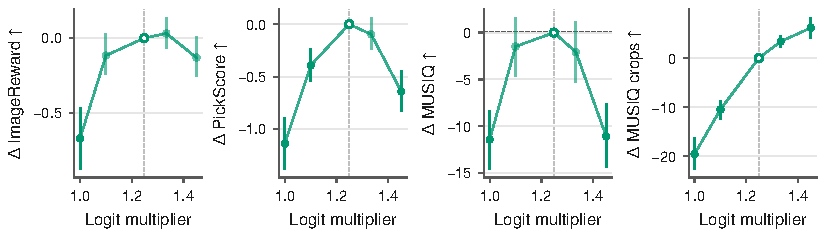
\includegraphics[width=\linewidth]{figs/strengthen/fs_sweep.pdf}
\caption{\textbf{Temperature sweep.} \tempsb{} at five logit multipliers fixed before generation, minus the reference $s^{0.16}$ (hollow mark, dashed vertical), on held-out rows 8 to 62 ($n=\N{st@s@n}$, seed 0). Whiskers are nominal 95\% paired intervals; pale marks cover zero. Reward models and full-frame MUSIQ fall on both sides of $s^{0.16}$, while crop MUSIQ keeps rising with the multiplier.}
\label{fig:fs-sweep}
\end{figure}
% Generated by paper/tables/strengthen_tables.py. Do not edit by hand.
\begin{table}[!htbp]
\centering
\caption{\textbf{Fresh prompts.} Means of \segaofficial{}, in the shaded column, and paired differences from it on 150 unseen Aesthetic-4K training captions ($n=150$, seed 0), with nominal 95\% intervals; $^{*}$ marks Holm-adjusted $p\le0.05$ over 50 tests (5 arms by 10 metrics). Bold marks the best entry for a metric when its interval separates it from \segaofficial. Key result: \dype{} is the only arm that beats \segaofficial{} under Holm on crop MUSIQ ($+2.32$) and CLIP-IQA ($+0.024$) while losing ImageReward ($-0.166$) and PickScore ($-0.38$); \tempsb{} ties ImageReward ($-0.011$) and loses crop CLIP-IQA and slope error under Holm.}
\label{tab:strengthen-fresh-arms}
\scriptsize
\setlength{\tabcolsep}{1.8pt}
% Generated by paper/tables/strengthen_tables.py. Do not edit by hand.
% Caption: \textbf{Fresh prompts.} Means of \segaofficial{}, in the shaded column, and paired differences from it on 150 unseen Aesthetic-4K training captions ($n=150$, seed 0), with nominal 95\% intervals; $^{*}$ marks Holm-adjusted $p\le0.05$ over 50 tests (5 arms by 10 metrics). Bold marks the best entry for a metric when its interval separates it from \segaofficial. Key result: \dype{} is the only arm that beats \segaofficial{} under Holm on crop MUSIQ ($+2.32$) and CLIP-IQA ($+0.024$) while losing ImageReward ($-0.166$) and PickScore ($-0.38$); \tempsb{} ties ImageReward ($-0.011$) and loses crop CLIP-IQA and slope error under Holm.
\begin{tabular}{@{}l>{\columncolor{papertint}}rrrrrr@{}}
\toprule
Metric & \hdr{\sega{}\\(released)} & \hdr{\sega{} base\\+\,temp.} & \hdr{\sega{}\\base} & \hdr{\ntk{}\\+\,temp.} & \hdr{\dype{}\\\phantom{x}} & \hdr{\ntk{}\\\phantom{x}} \\
\midrule
ImageReward$\uparrow$ & \refcell{0.667} & \dcellT{-0.011}{-0.055}{+0.035} & \dcellW{-0.875^{*}}{-1.022}{-0.723} & \dcellT{-0.042}{-0.093}{+0.008} & \dcellW{-0.166^{*}}{-0.250}{-0.084} & \dcellW{-0.923^{*}}{-1.077}{-0.768} \\
PickScore$\uparrow$ & \refcell{\mathbf{22.56}} & \dcellW{-0.07}{-0.13}{-0.01} & \dcellW{-1.05^{*}}{-1.22}{-0.89} & \dcellW{-0.12^{*}}{-0.18}{-0.05} & \dcellW{-0.38^{*}}{-0.51}{-0.26} & \dcellW{-1.05^{*}}{-1.22}{-0.89} \\
CLIP$\uparrow$ & \refcell{27.70} & \dcellT{-0.18}{-0.45}{+0.09} & \dcellW{-2.50^{*}}{-3.05}{-1.97} & \dcellT{-0.25}{-0.52}{+0.00} & \dcellT{-0.12}{-0.48}{+0.25} & \dcellW{-2.51^{*}}{-3.05}{-1.98} \\
MUSIQ$\uparrow$ & \refcell{44.99} & \dcellW{-1.56}{-2.72}{-0.43} & \dcellW{-10.28^{*}}{-12.15}{-8.33} & \dcellT{-0.76}{-1.99}{+0.49} & \dcellT{-0.65}{-1.99}{+0.74} & \dcellW{-10.48^{*}}{-12.46}{-8.53} \\
MUSIQ\textsubscript{crop}$\uparrow$ & \refcell{58.66} & \dcellT{-0.64}{-1.32}{+0.03} & \dcellW{-13.15^{*}}{-14.99}{-11.42} & \dcellT{-0.55}{-1.15}{+0.07} & \dcellB{\mathbf{+2.32}^{*}}{+1.41}{+3.25} & \dcellW{-13.00^{*}}{-14.75}{-11.29} \\
CLIP-IQA$\uparrow$ & \refcell{0.590} & \dcellT{-0.007}{-0.017}{+0.002} & \dcellW{-0.024}{-0.040}{-0.007} & \dcellW{-0.012}{-0.022}{-0.002} & \dcellB{\mathbf{+0.024}^{*}}{+0.011}{+0.036} & \dcellW{-0.021}{-0.038}{-0.003} \\
CLIP-IQA\textsubscript{crop}$\uparrow$ & \refcell{0.583} & \dcellW{-0.023^{*}}{-0.033}{-0.013} & \dcellW{-0.024}{-0.040}{-0.008} & \dcellW{-0.028^{*}}{-0.039}{-0.017} & \dcellT{+0.011}{-0.002}{+0.025} & \dcellW{-0.018}{-0.035}{-0.002} \\
Spec.\ err.$\downarrow$ & \refcell{1.133} & \dcellT{+0.005}{-0.035}{+0.038} & \dcellW{+0.469^{*}}{+0.344}{+0.608} & \dcellT{+0.014}{-0.028}{+0.050} & \dcellT{-0.042}{-0.101}{+0.011} & \dcellW{+0.434^{*}}{+0.294}{+0.582} \\
Slope err.$\downarrow$ & \refcell{0.220} & \dcellW{+0.016^{*}}{+0.006}{+0.026} & \dcellT{+0.013}{-0.016}{+0.042} & \dcellT{+0.012}{-0.003}{+0.026} & \dcellW{+0.016}{+0.000}{+0.031} & \dcellT{+0.008}{-0.020}{+0.038} \\
Tiling$\downarrow$ & \refcell{0.0644} & \dcellB{-0.0058}{-0.0094}{-0.0022} & \dcellT{-0.0107}{-0.0225}{+0.0004} & \dcellT{-0.0014}{-0.0057}{+0.0030} & \dcellT{+0.0090}{-0.0026}{+0.0214} & \dcellT{-0.0062}{-0.0175}{+0.0048} \\
\bottomrule
\end{tabular}

\end{table}

% Generated by paper/tables/strengthen_tables.py. Do not edit by hand.
\begin{table}[!htbp]
\centering
\caption{\textbf{Seed replication.} Held-out rows 8 to 194 ($n=187$ prompts): \segaofficial{} means over seeds 0 to 2 (shaded column) and paired differences of \tempsb{} minus \segaofficial. The first difference column averages seeds 0, 1 and 2 within each prompt before the paired bootstrap; $^{*}$ marks Holm-adjusted $p\le0.05$ over its 10 metrics and bold marks the better arm where its interval excludes zero. The other columns are sensitivity analyses without Holm marks. Key result: Averaged over seeds, \tempsb{} minus \segaofficial{} is $+0.021$ [$-0.004$, $+0.044$] on ImageReward and $-0.000$ [$-0.035$, $+0.037$] on PickScore, and $-2.00$ [$-2.74$, $-1.30$] on full-frame MUSIQ (Holm); every single seed gives the same MUSIQ verdict.}
\label{tab:strengthen-seeds}
\scriptsize
\setlength{\tabcolsep}{1.8pt}
% Generated by paper/tables/strengthen_tables.py. Do not edit by hand.
% Caption: \textbf{Seed replication.} Held-out rows 8 to 194 ($n=187$ prompts): \segaofficial{} means over seeds 0 to 2 (shaded column) and paired differences of \tempsb{} minus \segaofficial. The first difference column averages seeds 0, 1 and 2 within each prompt before the paired bootstrap; $^{*}$ marks Holm-adjusted $p\le0.05$ over its 10 metrics and bold marks the better arm where its interval excludes zero. The other columns are sensitivity analyses without Holm marks. Key result: averaged over seeds, \tempsb{} minus \segaofficial{} is $+0.021$ [$-0.004$, $+0.044$] on ImageReward and $-0.000$ [$-0.035$, $+0.037$] on PickScore, and $-2.00$ [$-2.74$, $-1.30$] on full-frame MUSIQ (Holm); every single seed gives the same MUSIQ verdict.
\begin{tabular}{@{}l>{\columncolor{papertint}}rrrrrr@{}}
\toprule
Metric & \hdr{\sega{} (rel.)\\seeds 0 to 2} & \hdr{Seeds\\0, 1, 2} & \hdr{Seeds\\1, 2} & \hdr{Seed\\0} & \hdr{Seed\\1} & \hdr{Seed\\2} \\
\midrule
ImageReward$\uparrow$ & \refcell{1.227} & \dcellT{+0.021}{-0.004}{+0.044} & \dcellT{+0.018}{-0.007}{+0.042} & \dcellT{+0.026}{-0.014}{+0.068} & \dcellT{+0.008}{-0.023}{+0.038} & \dcellT{+0.029}{-0.005}{+0.064} \\
PickScore$\uparrow$ & \refcell{23.10} & \dcellT{-0.00}{-0.04}{+0.04} & \dcellT{-0.01}{-0.06}{+0.03} & \dcellT{+0.03}{-0.03}{+0.09} & \dcellT{+0.01}{-0.05}{+0.07} & \dcellT{-0.04}{-0.10}{+0.02} \\
CLIP$\uparrow$ & \refcell{29.14} & \dcellT{-0.02}{-0.18}{+0.12} & \dcellT{-0.04}{-0.22}{+0.13} & \dcellT{+0.02}{-0.19}{+0.23} & \dcellT{-0.14}{-0.38}{+0.08} & \dcellT{+0.06}{-0.15}{+0.27} \\
MUSIQ$\uparrow$ & \refcell{\mathbf{45.34}} & \dcellW{-2.00^{*}}{-2.74}{-1.30} & \dcellW{-1.96}{-2.81}{-1.20} & \dcellW{-2.09}{-3.25}{-0.97} & \dcellW{-2.14}{-3.23}{-1.14} & \dcellW{-1.77}{-2.66}{-0.98} \\
MUSIQ\textsubscript{crop}$\uparrow$ & \refcell{58.40} & \dcellT{-0.19}{-0.69}{+0.30} & \dcellT{-0.23}{-0.79}{+0.35} & \dcellT{-0.11}{-0.71}{+0.48} & \dcellT{-0.22}{-0.89}{+0.46} & \dcellT{-0.23}{-0.86}{+0.46} \\
CLIP-IQA$\uparrow$ & \refcell{\mathbf{0.600}} & \dcellW{-0.007}{-0.013}{-0.000} & \dcellT{-0.005}{-0.012}{+0.002} & \dcellW{-0.009}{-0.018}{-0.001} & \dcellT{-0.007}{-0.015}{+0.001} & \dcellT{-0.004}{-0.012}{+0.004} \\
CLIP-IQA\textsubscript{crop}$\uparrow$ & \refcell{\mathbf{0.585}} & \dcellW{-0.014^{*}}{-0.021}{-0.007} & \dcellW{-0.013}{-0.020}{-0.005} & \dcellW{-0.017}{-0.025}{-0.008} & \dcellW{-0.014}{-0.023}{-0.005} & \dcellW{-0.012}{-0.020}{-0.003} \\
Spec.\ err.$\downarrow$ & \refcell{\mathbf{1.057}} & \dcellW{+0.045^{*}}{+0.029}{+0.061} & \dcellW{+0.050}{+0.033}{+0.068} & \dcellW{+0.034}{+0.015}{+0.052} & \dcellW{+0.054}{+0.035}{+0.074} & \dcellW{+0.046}{+0.026}{+0.066} \\
Slope err.$\downarrow$ & \refcell{\mathbf{0.199}} & \dcellW{+0.023^{*}}{+0.014}{+0.033} & \dcellW{+0.023}{+0.014}{+0.033} & \dcellW{+0.024}{+0.013}{+0.034} & \dcellW{+0.023}{+0.011}{+0.034} & \dcellW{+0.024}{+0.013}{+0.035} \\
Tiling$\downarrow$ & \refcell{0.0669} & \dcellB{\mathbf{-0.0060}^{*}}{-0.0085}{-0.0033} & \dcellB{-0.0056}{-0.0088}{-0.0024} & \dcellB{-0.0068}{-0.0106}{-0.0028} & \dcellT{-0.0033}{-0.0076}{+0.0011} & \dcellB{-0.0078}{-0.0123}{-0.0040} \\
\bottomrule
\end{tabular}

\end{table}

% Generated by paper/tables/strengthen_tables.py. Do not edit by hand.
\begin{table}[!htbp]
\centering
\caption{\textbf{Checkpoint by guidance.} Official \dype{} code on development rows 0 to 7 (seed 42, 28 steps, $4096^2$). Each entry is a ratio of whitened luminance power (radial power times $f^2$, Hann window) at one lattice bin with a period of 8 to 64 pixels: geometric mean over the 8 prompts with a 95\% bootstrap interval on the logs. The historical statistic picks the bin on the \fluxdev{} image and is biased upward; the shared bin is picked once per prompt from the mean log spectrum of all four cells. Descriptive development evidence, not a held-out test. Key result: \fluxdev{} carries more lattice power than \krea{} at both matched guidance values; raising guidance from 3.5 to 4.5 lowers it on \fluxdev{} while the \krea{} interval covers 1, so guidance modulates the lattice but does not create the checkpoint gap.}
\label{tab:strengthen-ckpt}
\scriptsize
\setlength{\tabcolsep}{1.8pt}
% Generated by paper/tables/strengthen_tables.py. Do not edit by hand.
% Caption: \textbf{Checkpoint by guidance.} Official \dype{} code on development rows 0 to 7 (seed 42, 28 steps, $4096^2$). Each entry is a ratio of whitened luminance power (radial power times $f^2$, Hann window) at one lattice bin with a period of 8 to 64 pixels: geometric mean over the 8 prompts with a 95\% bootstrap interval on the logs. The historical statistic picks the bin on the \fluxdev{} image and is biased upward; the shared bin is picked once per prompt from the mean log spectrum of all four cells. Descriptive development evidence, not a held-out test. Key result: \fluxdev{} carries more lattice power than \krea{} at both matched guidance values; raising guidance from 3.5 to 4.5 lowers it on \fluxdev{} while the \krea{} interval covers 1, so guidance modulates the lattice but does not create the checkpoint gap.
\begin{tabular}{@{}l rr@{}}
\toprule
Power ratio at the lattice bin & \hdr{Geometric\\mean} & \hdr{95\%\\interval} \\
\midrule
\multicolumn{3}{@{}l}{\emph{Historical F5 statistic, peak bin chosen on the \fluxdev{} image}} \\
\fluxdev/\krea, guidance $3.5$ & $12.0\times$ & $[7.8, 18.6]$ \\
\fluxdev/\krea, guidance $4.5$ & $7.4\times$ & $[4.5, 12.7]$ \\
\midrule
\multicolumn{3}{@{}l}{\emph{Shared bin, chosen on the mean of all four cells}} \\
\fluxdev/\krea, guidance $3.5$ & $11.6\times$ & $[7.5, 18.5]$ \\
\fluxdev/\krea, guidance $4.5$ & $6.7\times$ & $[4.2, 11.7]$ \\
Guidance $4.5/3.5$, \fluxdev & $0.52\times$ & $[0.41, 0.64]$ \\
Guidance $4.5/3.5$, \krea & $0.89\times$ & $[0.67, 1.11]$ \\
\bottomrule
\end{tabular}

\end{table}

% Generated by paper/tables/strengthen_tables.py. Do not edit by hand.
\begin{table}[!htbp]
\centering
\caption{\textbf{Default flow shift.} \segaofficial{} on development rows 0 to 7 (seed 0, 28 steps, guidance 4.5, $4096^2$) with the official shift ($\mu=1.15$, shaded) and with the diffusers default, which extrapolates $\mu$ to 11.55 at 65{,}536 image tokens. Means over 8 prompts, bold best; the last column is the paired difference with a nominal 95\% interval. Descriptive development evidence. Key result: the default shift worsens all ten metrics and lowers ImageReward by 3.70 [3.42, 3.96].}
\label{tab:strengthen-default-shift}
\scriptsize
\setlength{\tabcolsep}{1.8pt}
% Generated by paper/tables/strengthen_tables.py. Do not edit by hand.
% Caption: \textbf{Default flow shift.} \segaofficial{} on development rows 0 to 7 (seed 0, 28 steps, guidance 4.5, $4096^2$) with the official shift ($\mu=1.15$, shaded) and with the diffusers default, which extrapolates $\mu$ to 11.55 at 65{,}536 image tokens. Means over 8 prompts, bold best; the last column is the paired difference with a nominal 95\% interval. Descriptive development evidence. Key result: the default shift worsens all ten metrics and lowers ImageReward by 3.70 [3.42, 3.96].
\begin{tabular}{@{}l>{\columncolor{papertint}}rrr@{}}
\toprule
Metric & \hdr{Official\\$\mu=1.15$} & \hdr{Default\\$\mu=11.55$} & \hdr{Default\\$-$ official} \\
\midrule
ImageReward$\uparrow$ & \refcell{\mathbf{1.423}} & \refcell{-2.278} & \dcellW{-3.701}{-3.959}{-3.419} \\
PickScore$\uparrow$ & \refcell{\mathbf{23.41}} & \refcell{17.19} & \dcellW{-6.22}{-7.11}{-5.42} \\
CLIP$\uparrow$ & \refcell{\mathbf{30.32}} & \refcell{14.62} & \dcellW{-15.70}{-18.55}{-12.65} \\
MUSIQ$\uparrow$ & \refcell{\mathbf{42.49}} & \refcell{22.44} & \dcellW{-20.05}{-24.68}{-13.86} \\
MUSIQ\textsubscript{crop}$\uparrow$ & \refcell{\mathbf{58.23}} & \refcell{33.82} & \dcellW{-24.42}{-29.71}{-19.39} \\
CLIP-IQA$\uparrow$ & \refcell{\mathbf{0.557}} & \refcell{0.377} & \dcellW{-0.180}{-0.269}{-0.080} \\
CLIP-IQA\textsubscript{crop}$\uparrow$ & \refcell{\mathbf{0.580}} & \refcell{0.372} & \dcellW{-0.208}{-0.266}{-0.146} \\
Spec.\ err.$\downarrow$ & \refcell{\mathbf{0.857}} & \refcell{2.906} & \dcellW{+2.049}{+1.410}{+2.706} \\
Slope err.$\downarrow$ & \refcell{\mathbf{0.099}} & \refcell{0.499} & \dcellW{+0.400}{+0.256}{+0.542} \\
Tiling$\downarrow$ & \refcell{\mathbf{0.0894}} & \refcell{0.1329} & \dcellW{+0.0435}{+0.0259}{+0.0646} \\
\bottomrule
\end{tabular}

\end{table}

